% Resultados e Discussão — Lab03, Issue #42.
% TODOS os números vêm de macros \N... (artigo/gerado/numeros.tex) e das tabelas de artigo/gerado/, geradas por
% `python -m analysis.artigo_numeros` a partir de outputs/analise/ e outputs/sensitivity_dora.csv, que por sua vez
% são regenerados de data/metrics.csv (tag dataset-final). Não digitar números aqui.
% Conferência: `python -m analysis.artigo_numeros --check`.

\section{Resultados e Discussão}\label{sec:resultados}

Todas as análises partem de \texttt{data/metrics.csv} ($n = \NTotal$ repositórios, janela de
2025-10-02 a 2026-10-02). Descrevemos cada métrica por mediana e intervalo interquartil (IQR), e classificamos
com os cortes fixos da disciplina. As métricas dependem de proxies (release $\neq$ deploy; falha de CI
$\neq$ falha em produção), e o CFR~(b) é exploratório porque a heurística corretiva obteve F1 independente de
0,689, abaixo da meta de 0,70 (Seção~\ref{sec:heuristica}). A Tabela~\ref{tab:resumo} resume as seis
métricas; a Tabela~\ref{tab:hipoteses} confronta as hipóteses da Introdução com os resultados.

\begin{table}[ht]
\centering\small
\caption{Resumo das métricas por repositório: mediana, quartis, IQR e classe DORA. ``Classe (mediana)'' classifica
o valor da mediana; E/H/M/L é o número de repositórios em Elite/High/Medium/Low. Recuperação: apenas
repositórios com episódio concluído.}
\label{tab:resumo}
\resizebox{\linewidth}{!}{% Gerado por analysis/artigo_numeros.py a partir de outputs/analise/rq01_rq04_descritiva.csv. Não editar.
\begin{tabular}{llrrrrrll}
\hline
RQ & Métrica & $n$ & Mediana & Q1 & Q3 & IQR & Classe (mediana) & E/H/M/L \\ \hline
RQ01 & Deployment frequency (rel./sem.) & 300 & 0{,}36 & 0{,}19 & 0{,}77 & 0{,}58 & Medium & 6/55/143/96 \\
RQ02 & Lead time (a), por release (h) & 300 & 146{,}4 & 26{,}8 & 544{,}4 & 517{,}6 & High & 70/88/86/56 \\
RQ02 & Lead time (b), por commit (h) & 300 & 146{,}3 & 32{,}5 & 437{,}0 & 404{,}6 & High & 66/87/95/52 \\
RQ03 & CFR (a), proxy de CI (\%) & 300 & 5{,}7 & 2{,}4 & 14{,}1 & 11{,}7 & Elite & 229/40/17/14 \\
RQ03 & CFR (b), proxy de entrega (\%) & 299 & 20{,}0 & 4{,}1 & 46{,}5 & 42{,}4 & High & 121/67/33/78 \\
RQ04 & Recuperação (h) & 277 & 2{,}8 & 0{,}7 & 21{,}2 & 20{,}6 & High & 92/126/43/16 \\
\hline
\end{tabular}
}
\end{table}

\begin{table}[ht]
\centering\small
\caption{Hipóteses $\times$ resultados ($n = \NTotal$ repositórios).}
\label{tab:hipoteses}
\begin{tabular}{lp{3.2cm}p{4.4cm}l}
\hline
\textbf{H} & \textbf{Esperado} & \textbf{Observado} & \textbf{Confirmada?} \\
\hline
H1 & Mediana em \textit{Medium}, cauda de alta frequência &
  Mediana \NDfMed{} rel./sem. (\textit{Medium}); \NDfClasseHigh\% \textit{High} e \NDfClasseElite\% \textit{Elite} &
  Sim \\
H2 & LT(b) $\ll$ LT(a) &
  Medianas entre repositórios iguais (\NLtaMed{} h e \NLtbMed{} h); por repositório, a razão LT(a)/LT(b) tem mediana \NRazMed{} e IQR \NRazQum--\NRazQtres &
  Não \\
H3 & CFR(a) $>$ CFR(b); CFR(a) entre 10\% e 30\% &
  CFR(a) \NCfraMed\%; CFR(b) \NCfrbMed\% &
  Não \\
H4 & Mediana de 1 h a 1 dia; parcela relevante de episódios censurados &
  Mediana \NRecMed{} h; censurados: \NCensPct\% dos episódios &
  Parcial \\
H5 & Correlação fraca ou levemente negativa entre DF e CFR &
  CFR(a): $\rho = \NRhoA$; CFR(b): $\rho = \NRhoB$ &
  Parcial \\
H6 & Linguagem e tipo mais fortes que popularidade; idade e contribuidores com efeito pequeno &
  \NSeisSig{} de \NSeisTestes{} testes significativos após Holm: idade (4), contribuidores (2), linguagem (2); tipo e popularidade, nenhum &
  Parcial \\
H7 & Mais de 30\% mudam de categoria; $\kappa$ no máximo moderado &
  C1$\times$C2: \NSensUmDoisPct\%, $\kappa = \NSensUmDoisKappa$; C1$\times$C3: \NSensUmTresPct\%, $\kappa = \NSensUmTresKappa$ &
  Parcial \\
\hline
\end{tabular}
\end{table}

\subsection{RQ01 --- Frequência de deploy}

A mediana foi de \textbf{\NDfMed{} releases/semana} (Q1 = \NDfQum; Q3 = \NDfQtres; IQR = \NDfIqr;
$n = \NDfN$), isto é, pouco mais de uma release a cada três semanas. A distribuição é assimétrica à direita
(Figura~\ref{fig:rq01}). Pelos cortes da disciplina, \NDfClasseElite\% dos repositórios são \textit{Elite}
($\geq 7$ por semana), \NDfClasseHigh\% \textit{High}, \NDfClasseMedium\% \textit{Medium} e
\NDfClasseLow\% \textit{Low} ($<$ 1 por mês). A classe \textit{geral} C1, que combina as quatro métricas,
distribui-se de outra forma: \NUmClasseElite\% \textit{Elite}, \NUmClasseHigh\% \textit{High},
\NUmClasseMedium\% \textit{Medium} e \NUmClasseLow\% \textit{Low}.

A H1 se confirma: a mediana cai em \textit{Medium}, e \NDfClasseHigh\% mais \NDfClasseElite\% publicam ao menos
uma release por semana. Como a unidade é a release publicada, o resultado descreve ritmo de versões, não
necessariamente de deploys em produção.

\begin{figure}[ht]
\centering
\includegraphics[width=.7\linewidth]{figs/rq01_df.png}
\caption{RQ01: deployment frequency por repositório (escala log); linha = mediana, faixa = IQR.}
\label{fig:rq01}
\end{figure}

\subsection{RQ02 --- Lead time for changes}

A mediana entre repositórios do \textit{lead time} por release, LT(a), foi de \textbf{\NLtaMed{} h}
($\approx$ \NLtaDias{} dias; Q1 = \NLtaQum{} h; Q3 = \NLtaQtres{} h), e a do LT(b), por commit, de
\textbf{\NLtbMed{} h} (Q1 = \NLtbQum{} h; Q3 = \NLtbQtres{} h). Ambas caem em \textit{High}. As duas
medianas coincidem, o que contraria a H2 (esperávamos LT(b) $\ll$ LT(a)), mas essa coincidência é do
\emph{agregado}: por repositório as variantes divergem (Figura~\ref{fig:rq02}). A razão LT(a)/LT(b) tem mediana
\NRazMed{} e IQR \NRazQum--\NRazQtres; LT(a) supera o dobro de LT(b) em \NRazAdobroB\% dos repositórios, LT(b)
supera o dobro de LT(a) em \NRazBdobroA\%, e só \NRazMeio\% ficam entre metade e o dobro (Wilcoxon pareado,
$p$ \NRazWilcoxonP).

As variantes medem coisas diferentes. LT(a) é, em cada release, o tempo do commit \emph{mais antigo}, e o
repositório fica com a mediana desses máximos; LT(b) junta os commits de todas as releases e toma a mediana,
de modo que releases com muitos commits pesam mais. Um commit antigo ``esquecido'' numa release eleva LT(a)
dessa release sem mover muito a mediana por commit, e é essa a explicação esperada para LT(a) $>$ LT(b); mas
\NRazAmenorB\% dos repositórios têm LT(a) $<$ LT(b), o que o commit esquecido não explica. Não testamos
nenhuma explicação causal: o CSV só traz as medianas por repositório,
e o lead time de cada commit está no cache da coleta, que não é versionado. Registramos apenas o tamanho e o
sentido da divergência (\texttt{rq02\_divergencia.csv}). O número de releases avaliadas explica pouco dela
(Spearman entre log da razão e esse número: $\rho = \NRazRho$, $p = $ \NRazRhoP).

\begin{figure}[ht]
\centering
\includegraphics[width=.6\linewidth]{figs/rq02_lead_time.png}\\[2pt]
\includegraphics[width=\linewidth]{figs/rq02_divergencia.png}
\caption{RQ02: LT(a) e LT(b) por repositório (acima); dispersão LT(a)$\times$LT(b) e histograma de
log$_2$(LT(a)/LT(b)) (abaixo).}
\label{fig:rq02}
\end{figure}

\subsection{RQ03 --- Change failure rate}

O CFR~(a), proxy de CI, teve mediana de \textbf{\NCfraMed\%} (Q1 = \NCfraQum\%; Q3 = \NCfraQtres\%;
$n = \NCfraN$). O CFR~(b), proxy de entrega, teve mediana de \textbf{\NCfrbMed\%} (Q1 = \NCfrbQum\%;
Q3 = \NCfrbQtres\%; IQR = \NCfrbIqr{} p.p.; $n = \NCfrbN$; um repositório tem menos de duas releases na
janela e fica indefinido). A H3 é refutada nos dois pontos: o CFR(a) ficou abaixo da faixa de 10\%--30\%, e
o CFR(b) superou o CFR(a).

As duas variantes medem eventos diferentes. O CFR(a) conta \emph{execuções de CI} do \textit{default branch} que
falharam; uma falha de pipeline (teste instável, lint, ambiente) não equivale a uma falha em produção, e
muitas falhas nunca chegam a uma release. O CFR(b) conta \emph{releases} seguidas, em até 7 dias, de uma release
classificada como corretiva pela heurística v12, cuja precisão e recall são imperfeitos (F1 independente de
0,689); o valor reflete tanto correções reais quanto erros do proxy. Por isso tratamos o CFR(b) como
exploratório, e a diferença entre as variantes como ameaça de construto (Seção de Ameaças).

\subsection{RQ04 --- Tempo de recuperação}\label{sec:resultados-rq04}

O tempo mediano de recuperação foi de \textbf{\NRecMed{} h} (Q1 = \NRecQum{} h; Q3 = \NRecQtres{} h;
IQR = \NRecIqr{} h; $n = \NRecN$ repositórios com episódio concluído), classe \textit{High}.

\textbf{Censura.} Dos \NCensTot{} episódios de falha, \NCensEp{} (\NCensPct\%) não foram concluídos na janela e
são \emph{censurados}. Entre os \NCensReposCom{} repositórios com algum episódio, a mediana da proporção de
censurados é \NCensRepoMed\% (Q3 = \NCensRepoQtres\%), e \NCensReposAlgum{} repositórios têm ao menos um
episódio censurado (Figura~\ref{fig:rq04}). Os episódios censurados não entram na mediana de recuperação; são
contados à parte. Dos \NRecSemValor{} repositórios sem valor de recuperação, \NCensReposSem{} não tiveram
nenhum episódio de falha e \NCensSoCens{} só tiveram episódios censurados; esses seis estão fora da mediana, o
que tende a subestimar o tempo de recuperação, embora o efeito seja pequeno dado o volume de censura.

\textbf{Decisão metodológica.} O enunciado inicia o episódio na ``primeira falha após um sucesso''. O código
também abre um episódio quando a primeira execução válida de um workflow na janela é uma falha, sem sucesso
anterior (Seção de Metodologia, lacuna L09).

A H4 se confirma só em parte: a mediana está entre 1 hora e 1 dia, mas a censura é pequena
(\NCensPct\% dos episódios), bem abaixo da ``parcela relevante'' esperada. O valor baixo sugere correção rápida
de falhas de CI nesses projetos, sujeito à ressalva sobre censura acima.

\begin{figure}[ht]
\centering
\includegraphics[width=.7\linewidth]{figs/rq04_recuperacao.png}\\[2pt]
\includegraphics[width=.7\linewidth]{figs/rq04_censura.png}
\caption{RQ04: tempo de recuperação por repositório (acima, escala log) e proporção de episódios censurados por
repositório (abaixo).}
\label{fig:rq04}
\end{figure}

\subsection{RQ05 --- Frequência de deploy $\times$ CFR}

Com o CFR(a), o coeficiente de Spearman foi $\rho = \NRhoA$ ($p = $ \NRhoPA; IC 95\% \NRhoIcA;
$n = \NRhoNA$): sem relação monotônica detectável. Os intervalos usam a transformação $z$ de Fisher com erro-padrão de Bonett e Wright~\cite{bonett2000spearman}. Com o CFR(b), $\rho = \NRhoB$ ($p$ \NRhoPB; IC 95\%
\NRhoIcB; $n = \NRhoNB$): correlação positiva forte (Figura~\ref{fig:rq05}). A H5 se confirma só para a
variante (a).

Esse resultado não refuta a tese DORA de que velocidade e estabilidade não são um \textit{trade-off}, e
correlação não implica causalidade. O CFR(b) está acoplado mecanicamente à frequência de releases: quanto mais
releases, mais chances de existir uma corretiva em 7 dias, e o denominador pequeno de repositórios com poucas
releases produz muitos zeros. Restringindo a repositórios com ao menos 20 releases avaliadas o coeficiente cai
para $\rho = \NRhoBVinte$ ($n = \NRhoBVinteN$), mas essa restrição também reduz a faixa de DF, e o diagnóstico
não separa os efeitos. A idade confunde a leitura (RQ06): os repositórios mais jovens publicam mais e têm CFR(b)
mais alto. Como o proxy é exploratório, o resultado (b) indica um possível artefato, não evidência contra a
tese DORA; e o resultado (a), sem relação, é compatível com ela.

\begin{figure}[ht]
\centering
\includegraphics[width=.7\linewidth]{figs/rq05_df_cfr_a.png}\\[2pt]
\includegraphics[width=.7\linewidth]{figs/rq05_df_cfr_b.png}
\caption{RQ05: DF (escala log) $\times$ CFR(a) (acima) e CFR(b) (abaixo); linha = mediana do CFR por faixa de DF.}
\label{fig:rq05}
\end{figure}

\subsection{RQ06 --- Características dos repositórios e métricas DORA}

Testamos cinco fatores (linguagem, popularidade, contribuidores, idade, tipo do projeto) contra as seis
métricas, num total de \NSeisTestes{} testes. Todos os fatores têm três ou mais grupos
(linguagem com 7 grupos, ``Outras'' para linguagens com menos de 15 repositórios; quartis; tipo em 3 classes
com $n = \NTipoN$ rotulados), então todos usaram Kruskal-Wallis; o ramo de Mann-Whitney e o $\delta$ de Cliff~\cite{cliff1993dominance}
não foram exercitados com dados reais, e o $\delta$ (magnitude conforme Romano et al.~\cite{romano2006appropriate}) aparece só como contraste descritivo Q4$\times$Q1 em
\texttt{rq06\_testes.csv}. Os p-valores foram corrigidos por Holm~\cite{holm1979sequentially} sobre os \NSeisTestes{} testes, e o tamanho
de efeito é $\varepsilon^2 = H/(n-1)$, interpretado como pequeno ($0{,}01$ a $<0{,}08$), médio ($<0{,}26$) ou grande, pela escala de
Mangiafico~\cite{mangiafico2016handbook}, que o próprio autor descreve como orientação, não como padrão universal;
usamos ``desprezível'' para $<0{,}01$, rótulo nosso.

Após Holm, \textbf{\NSeisSig{} associações permaneceram significativas} (Tabela~\ref{tab:rq06} e Figura~\ref{fig:rq06}), todas de
efeito médio:
\begin{itemize}
  \item \textbf{Idade} (4 associações): os repositórios mais jovens (Q1) publicam mais (DF mediana \NIdadeDfQum{}
  contra \NIdadeDfQquatro{} rel./sem. no Q4), têm LT(a) menor (\NIdadeLtaQum{} h contra \NIdadeLtaQquatro{} h) e
  CFR(b) maior (\NIdadeCfrbQum\% contra \NIdadeCfrbQquatro\%). A associação com o CFR(b) acompanha a de DF,
  em linha com o acoplamento discutido na RQ05.
  \item \textbf{Contribuidores} (2): mais contribuidores, LT maior (LT(a) mediana de \NContribLtaQum{} h no Q1 contra
  \NContribLtaQquatro{} h no Q4).
  \item \textbf{Linguagem} (2): LT(a) e recuperação; Rust tem os menores LT(a), e JavaScript a recuperação mais
  rápida; C++ tem os maiores LT(a) entre as linguagens nomeadas.
\end{itemize}
Popularidade (menor $p_{\mathrm{Holm}}$ = \NPopMinPHolm) e tipo do projeto não foram significativos; no tipo,
o $n = \NTipoN$ limita o poder. A H6 é parcial: linguagem pesa mais que popularidade, como esperado, mas o tipo
não se destaca, e idade e contribuidores têm efeito médio, não pequeno. São associações, não causas: idade, número de contribuidores e linguagem podem
estar associados a outras características não medidas dos projetos.

\begin{table}[ht]
\centering\small
\caption{RQ06: associações significativas após Holm (Kruskal-Wallis; $\varepsilon^2 = H/(n-1)$). A tabela
completa, com os \NSeisTestes{} testes, está em \texttt{outputs/analise/rq06\_testes.csv}.}
\label{tab:rq06}
\resizebox{\linewidth}{!}{% Gerado por analysis/artigo_numeros.py a partir de outputs/analise/rq06_testes.csv. Não editar.
\begin{tabular}{llrrrrl}
\hline
Fator & Métrica & $n$ & $H$ & $p_{\mathrm{Holm}}$ & $\varepsilon^2$ & Magnitude \\ \hline
Idade & Lead time (a) por release & 300 & 64{,}8 & $<0{,}001$ & 0{,}217 & médio \\
Idade & Lead time (b) por commit & 300 & 51{,}2 & $<0{,}001$ & 0{,}171 & médio \\
Idade & CFR (b) proxy de entrega & 299 & 40{,}3 & $<0{,}001$ & 0{,}135 & médio \\
Idade & Deployment frequency & 300 & 36{,}2 & $<0{,}001$ & 0{,}121 & médio \\
Contribuidores & Lead time (a) por release & 300 & 33{,}8 & $<0{,}001$ & 0{,}113 & médio \\
Contribuidores & Lead time (b) por commit & 300 & 26{,}0 & $<0{,}001$ & 0{,}087 & médio \\
Linguagem & Lead time (a) por release & 298 & 24{,}9 & $0{{,}}0087$ & 0{,}084 & médio \\
Linguagem & Tempo de recuperação & 276 & 22{,}2 & $0{{,}}025$ & 0{,}081 & médio \\
\hline
\end{tabular}
}
\end{table}

\begin{figure}[ht]
\centering
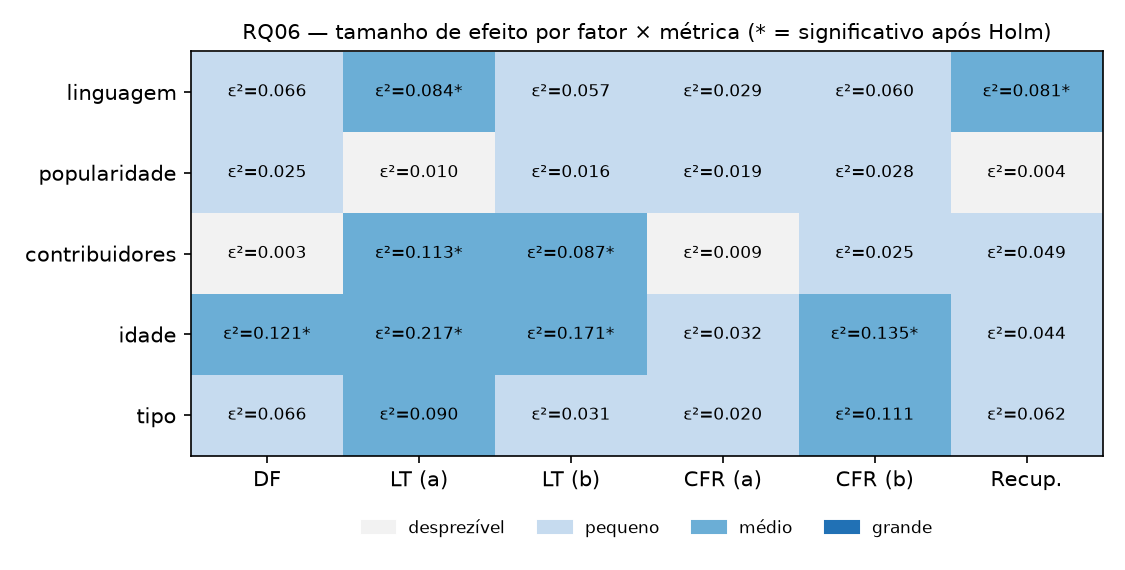
\includegraphics[width=.85\linewidth]{figs/rq06_efeitos.png}
\caption{RQ06: tamanho de efeito ($\varepsilon^2$) por fator e métrica.}
\label{fig:rq06}
\end{figure}

\subsection{RQ07 --- Sensibilidade das classificações DORA}

Comparamos três combinações (C1: release, LT(a), CFR(a); C2: release+pré-release, LT(b), CFR(b); C3: tag,
LT(b), CFR(a)). A Tabela~\ref{tab:rq07} e a Figura~\ref{fig:rq07} mostram a mudança de categoria e o $\kappa$
linear ponderado de cada par (categorias codificadas de 1 a 4, em ordem ordinal).

\begin{table}[ht]
\centering\small
\caption{RQ07: mudança de categoria geral e $\kappa$ de Cohen ponderado linear~\cite{cohen1968weighted} por par de combinações.}
\label{tab:rq07}
% Gerado por analysis/artigo_numeros.py a partir de outputs/sensitivity_dora.csv. Não editar.
\begin{tabular}{lrrrr}
\hline
Par & $n$ & Mudaram & \% que mudou & $\kappa$ linear \\ \hline
C1$\times$C2 & 300 & 121 & 40{,}3 & 0{,}46 \\
C1$\times$C3 & 300 & 67 & 22{,}3 & 0{,}72 \\
C2$\times$C3 & 300 & 88 & 29{,}3 & 0{,}61 \\
\hline
\end{tabular}

\end{table}

\begin{figure}[ht]
\centering
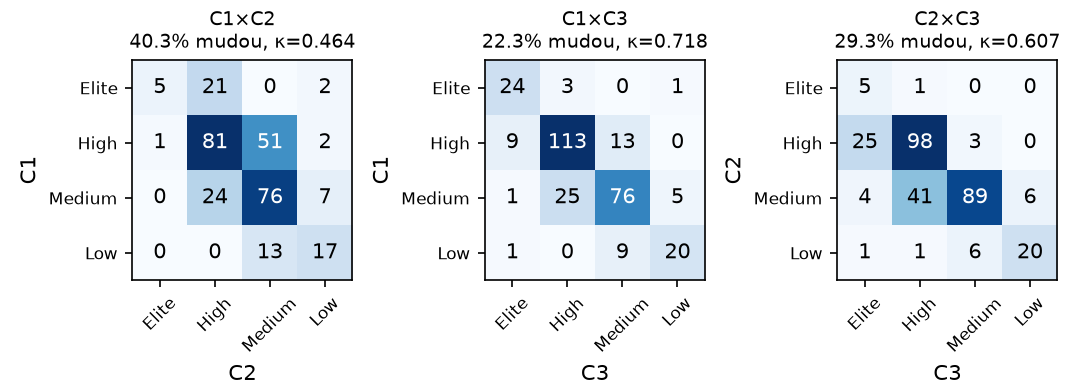
\includegraphics[width=\linewidth]{figs/sensitivity_transicao.png}
\caption{RQ07: matrizes de transição entre combinações (linha = primeira combinação; coluna = segunda).}
\label{fig:rq07}
\end{figure}

O par C1$\times$C2 muda em \NSensUmDoisPct\% dos repositórios ($\kappa = \NSensUmDoisKappa$, moderado), o que
confirma a H7; C1$\times$C3 muda em \NSensUmTresPct\% ($\kappa = \NSensUmTresKappa$) e C2$\times$C3 em
\NSensDoisTresPct\% ($\kappa = \NSensDoisTresKappa$), ambos substanciais, abaixo do limiar de 30\% da hipótese.

\textbf{Limitações.} Em C2 e C3 só a unidade do DF muda de fato (pré-releases, tags); LT(b) e CFR(b) seguem
calculados sobre releases (Seção de Metodologia). Repositórios sem episódio de recuperação são classificados com
três métricas (\NParcialCUm, \NParcialCDois{} e \NParcialCTres{} repositórios em C1, C2 e C3).

\textbf{Robustez das RQ01--RQ06.} A maior discordância está em C1$\times$C2, que troca CFR(a) por CFR(b) além da
unidade de deploy. Isso é coerente com a RQ03 e a RQ05, em que as duas variantes de CFR têm níveis e
correlações com a DF muito diferentes: as conclusões sobre CFR dependem da definição escolhida, e a sobre
DF$\times$CFR(b) é a menos robusta. As associações de LT da RQ06 (idade e contribuidores) aparecem tanto em LT(a)
quanto em LT(b), logo não dependem dessa escolha. A RQ01 depende da unidade de deploy (em C1$\times$C3, que muda
essencialmente a unidade do DF, \NSensUmTresPct\% dos repositórios mudam de classe geral). A RQ04 não tem
variante nas combinações. A análise ampliada (\texttt{sensitivity\_ampliada}) tem sete variações, das quais só quatro
reclassificam de fato (janela do CFR(b) e cortes $\pm 10\%$): mudam \NAmpInfMinPct\% a \NAmpInfMaxPct\% dos
repositórios, com $\kappa \geq \NAmpInfKappaMin$. As outras três (mínimo de releases e exclusão por censura) dão
0\% por construção, pois comparam o conjunto com um subconjunto dele mesmo, e não contam como evidência de
robustez. Assim, a classificação é estável a pequenas perturbações dos cortes, mas depende da unidade de deploy
e da variante de CFR.

\subsection{RQ08 --- Rework rate (bônus)}

A \textit{rework rate} --- proporção de releases de deploy corretivas na janela --- teve mediana de
\textbf{\NRwMed\%} (Q1 = \NRwQum\%; Q3 = \NRwQtres\%; $n = \NRwN$), contra \NRwCfrbMed\% do CFR(b) no
subconjunto pareado. Três repositórios ficam fora da RQ08: dois sem rótulos extraídos do cache e um cujos
contadores divergem do \texttt{metrics.csv} atual (os rótulos foram extraídos antes da regeneração do dataset
e não podem ser refeitos sem o cache). A diferença pareada (rework $-$ CFR(b)) tem mediana 0, mas IQR de
\NRwDifIqr{} p.p. (de \NRwDifQum{} a \NRwDifQtres{} p.p.) e Wilcoxon pareado com $p = $ \NRwWilcoxonP, e a
correlação entre as duas é moderada ($\rho = \NRwSpearman$). Portanto as medidas não são equivalentes: o CFR(b)
conta a release que \emph{precisou} de correção, e o rework a release que \emph{é} correção, sem exigir antecedente
em 7 dias nem censura. Ambas usam a mesma heurística v12 e herdam a sua imprecisão.
